%% LyX 2.2.2 created this file.  For more info, see http://www.lyx.org/.
%% Do not edit unless you really know what you are doing.
%\documentclass[english,conference,onecolumn]{IEEEtran}
\documentclass[english]{article}
\usepackage{spconf}
\usepackage{array}
\usepackage[T1]{fontenc}
\usepackage[utf8]{inputenc}
\usepackage{geometry}
\usepackage{algorithmic}
\usepackage{varwidth}
\usepackage{listings}
\geometry{verbose,tmargin=2cm,bmargin=2cm,lmargin=2cm,rmargin=2cm}
\usepackage{amsmath}
\usepackage{graphicx}
\usepackage{float}
\usepackage{babel}
\newfloat{algorithm}{tbp}{loa}
\floatname{algorithm}{Algorithm}


%\ninept\name{Jean-Marc Valin, Steinar Midtskogen}\address{Mozilla Corporation\\Mountain View, CA, USA}
\ninept
\twoauthors
{Steinar Midtskogen}{Cisco Systems Inc.\\Lysaker, Norway\\\texttt{stemidts@cisco.com}}
{Jean-Marc Valin}{Mozilla Corporation\\Mountain View, CA, USA\\\texttt{jmvalin@jmvalin.ca}}

\makeatletter

\newcolumntype{C}{>{\centering\arraybackslash}p{0.8em}}
\newcolumntype{X}{>{\centering\arraybackslash}p{10.5em}}

%%%%%%%%%%%%%%%%%%%%%%%%%%%%%% LyX specific LaTeX commands.
%% Because html converters don't know tabularnewline
\providecommand{\tabularnewline}{\\}

%%%%%%%%%%%%%%%%%%%%%%%%%%%%%% User specified LaTeX commands.
\usepackage{color}
\usepackage{url}
\usepackage[pdfpagemode=None,pdfstartview=FitH,pdfview=FitH,colorlinks=true,pdftitle=The AV1 Constrained Directional Enhancement Filter,pdfauthor=Jean-Marc Valin]{hyperref}

\makeatother

\begin{document}

\title{The AV1 Constrained Directional Enhancement Filter (CDEF)}

\maketitle
\begin{abstract}
This paper presents the constrained directional enhancement filter
designed for the AV1 royalty-free video codec. The filter is based on
a non-linear low-pass filter and is designed for vectorization
efficiency. It takes into account the direction of edges and patterns
being filtered. The filter works by identifying the direction of each
block and then adaptively filtering with a high degree of control over
the filter strength along the direction and across it.  The proposed
enhancement filter is shown to improve the quality of the
Alliance for Open Media (AOM) AV1 video codec in particular in low
complexity configurations.
\end{abstract}

\begin{keywords}enhancement filter, directional filter, AV1\end{keywords}

\section{Introduction}
\label{sec:intro}

The main goal of the constrained directional enhancement filter (CDEF)
is to filter out coding artifacts while
retaining the details of the image. In HEVC, the
Sample Adaptive Offset~(SAO)~\cite{HEVC-SAO} algorithm achieves a similar goal by defining
signal offsets for different classes of pixels. Unlike SAO, the
approach we take in AV1 is that of a non-linear spatial filter.  From
the very beginning, the design of the filter was constrained to be
easily vectorizable (i.e. implementable with SIMD operations), which
was not the case for other non-linear filters like the median
filter~\cite{Median} and the bilateral filter~\cite{Bilateral}.

The CDEF design originates from the following observations.
The amount of ringing artifacts in a coded image tends to be roughly proportional
to the quantization step size. The amount of detail is a property
of the input image, but the smallest detail actually retained in the
quantized image tends to also be proportional to the quantization
step size. For a given quantization step size, the amplitude of the
ringing is generally less than the amplitude of the details.

CDEF works by identifying the
direction of each block (Sec.~\ref{sec:direction-search}) and then adaptively filtering along the
identified direction (Sec.~\ref{sec:nonlinear-lowpass}) and also to a lesser degree along directions 45
degrees off the identified direction.  The filter strength along the
direction and 45 degrees off it can be signalled separately, which
allows a high degree of control over the blurring (Sec.~\ref{sec:signaling}).
Sec.~\ref{sec:encoder-search} demonstrates an efficient encoder search, with
results presented in Sec.~\ref{sec:results}.

\section{Direction Search}
\label{sec:direction-search}

We start by describing the direction search. The search operates on the
reconstructed pixels, just after the deblocking is applied. Since
those pixels are available to the decoder, no signalling is required
for the directions.
The direction search operates on $8\times8$ blocks, which is
fine enough to adequately handle non-straight edges,
while being large enough to reliably estimate directions when applied
to a quantized image. Having a constant direction over an $8\times8$
region also makes vectorization of the filter easier.

For each block we want to determine the direction that best matches
the pattern in the block. This is done by minimizing the sum of squared
differences (SSD) between the quantized block and a perfectly directional
block. A perfectly directional block is a block for which each line
along a certain direction has a constant value. For each direction,
we assign a line number $k$ to each pixel, as shown in Fig.~\ref{fig:Lines-for-direction}. 

\begin{figure}
\centering{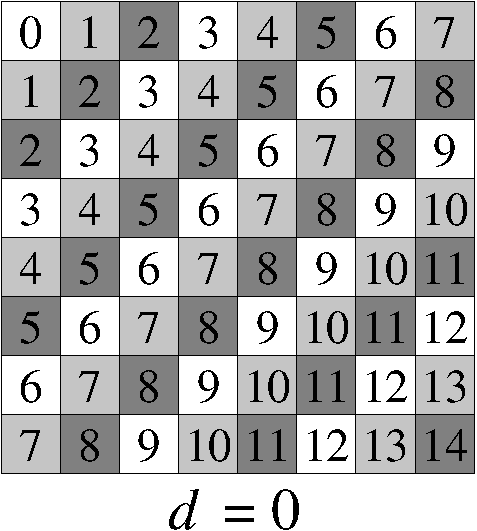
\includegraphics[width=0.24\columnwidth]{dlines0}\hspace{.35em}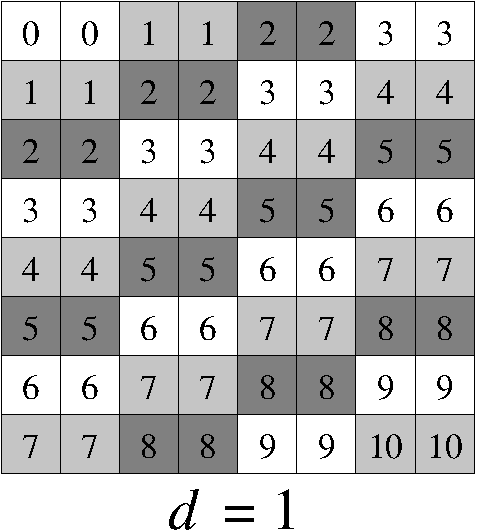
\includegraphics[width=0.24\columnwidth]{dlines1}\hspace{.35em}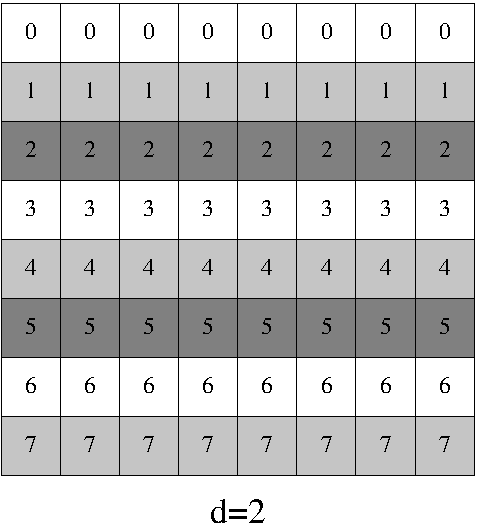
\includegraphics[width=0.24\columnwidth]{dlines2}\hspace{.35em}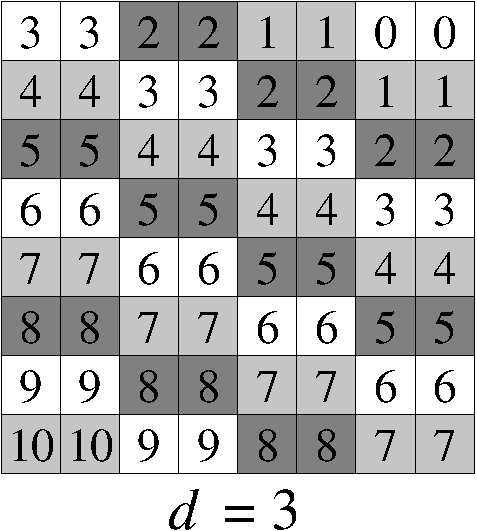
\includegraphics[width=0.24\columnwidth]{dlines3}}

\vspace{.5em}

\centering{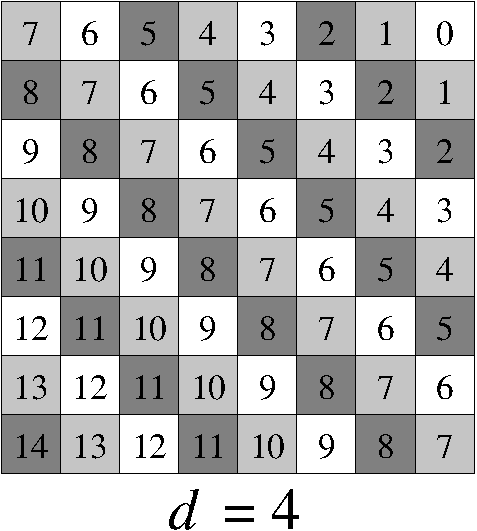
\includegraphics[width=0.24\columnwidth]{dlines4}\hspace{.35em}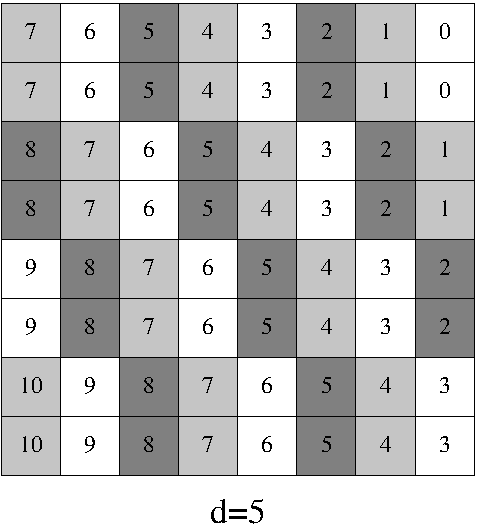
\includegraphics[width=0.24\columnwidth]{dlines5}\hspace{.35em}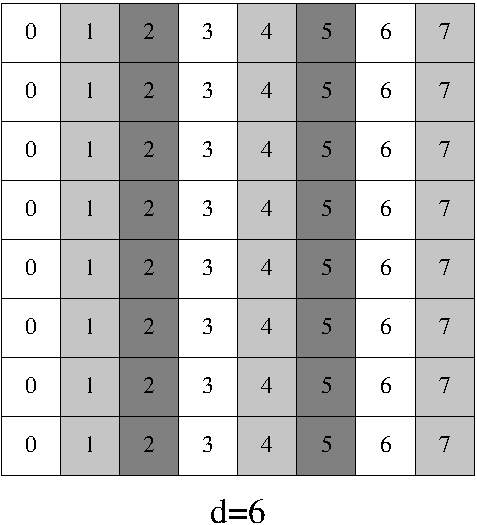
\includegraphics[width=0.24\columnwidth]{dlines6}\hspace{.35em}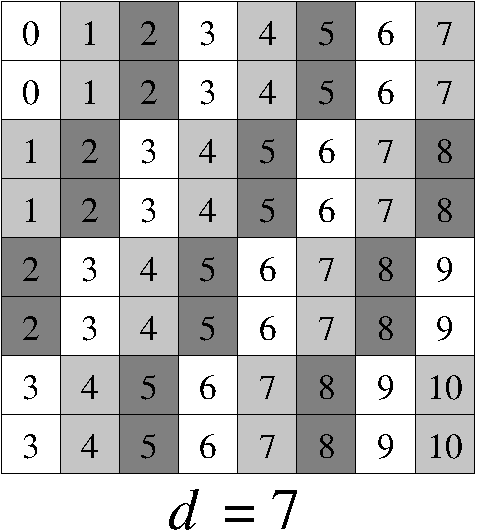
\includegraphics[width=0.24\columnwidth]{dlines7}}\caption{Line number $k$ for pixels following direction $d=0:7$ in an $8\times8$
block.\label{fig:Lines-for-direction}}
\end{figure}

For each direction $d$, the pixel average for line $k$ is determined
by:
\begin{equation}
\mu_{d,k}=\frac{1}{N_{d,k}}\sum_{p\in P_{d,k}}x_{p}\ ,\label{eq:pixel-average}
\end{equation}
where $x_{p}$ is the value of pixel $p$, $P_{d,k}$ is the set of
pixels in line $k$ following direction $d$ and $N_{d,k}$ is the
cardinality of $P_{d,k}$ (for example, in Fig.~\ref{fig:Lines-for-direction},
$N_{1,0}=2$ and $N_{1,4}=8$). The SSD is then defined as:
\begin{equation}
E_{d}^{2}=\sum_{k}\left[\sum_{p\in P_{d,k}}\left(x_{p}-\mu_{d,k}\right)^{2}\right]\ .\label{eq:direction-variance0}
\end{equation}

Substituting (\ref{eq:pixel-average}) into (\ref{eq:direction-variance0}) and
simplifying results in
\begin{equation}
E_{d}^{2}= \sum_{p}x_{p}^{2}-\sum_{k}\frac{1}{N_{d,k}}\left(\sum_{p\in P_{d,k}}x_{p}\right)^{2}\ .\label{eq:direction-variance1}
\end{equation}
 Note that the simplifications leading to (\ref{eq:direction-variance1})
are the same as to those allowing a variance to be computed as $\sigma_{x}^{2}=\frac{\sum x^{2}}{N}-\frac{\left(\sum x\right)^{2}}{N^2}$.
Considering that the first term of (\ref{eq:direction-variance1})
is constant with respect to $d$, we simply find the optimal direction
$d_{opt}$ by maximizing the second term:
\begin{equation}
d_{opt}=\max_{d}s_{d}\,,\label{eq:direction-variance2}
\end{equation}
where 
\begin{equation}
s_{d}=\sum_{k}\frac{1}{N_{d,k}}\left(\sum_{p\in P_{d,k}}x_{p}\right)^{2}\ .\label{eq:direction-variance3}
\end{equation}

We can avoid the division in (\ref{eq:direction-variance3}) by multiplying
$s_{d}$ by 840, the least common multiple of the possible $N_{d,k}$
values ($1\le N_{d,k}\le8$). When using 8\nobreakdash-bit pixel
data (for higher bit depths, we downscale to 8~bits), and centering
the values such that $-128\le x_{p}\le127$, then $840s_{d}$ and
all calculations leading to that value fit in a 32\nobreakdash-bit
signed integer.

Fig. \ref{fig:Example-of-direction} shows an example of a direction
search for an $8\times8$ block containing a line. 
The step-by-step process is described in algorithm~\ref{cap:direction-search}.  The search is only
done for the luma component, and the direction found in this search
is used for the chroma components.

In total, the search for all 8 directions requires the following
arithmetic operations:
\begin{enumerate}
\item The pixel accumulations in equation (\ref{eq:direction-variance3})
can be implemented with 294 additions (reusing partial sums of adjacent pixels).
\item The accumulations result in 90 line sums. Each is squared, requiring 90 multiplies.
\item Multiplying and summing the squared line sums to compute all $s_d$ values can be
simplified to 34 multiplies and 82 additions.
\item The resulting $s_d$ values are compared to find the largest value. 
\end{enumerate}

The total is 376~additions, 124~multiplies and 7 comparisons. That is about 1/3
fewer operations than an 8x8 DCT of the same size. The code can be efficiently vectorized,
with a small penalty due to the diagonal alignment, resulting in a completely similar to
that of a DCT.

\begin{figure}
\centering{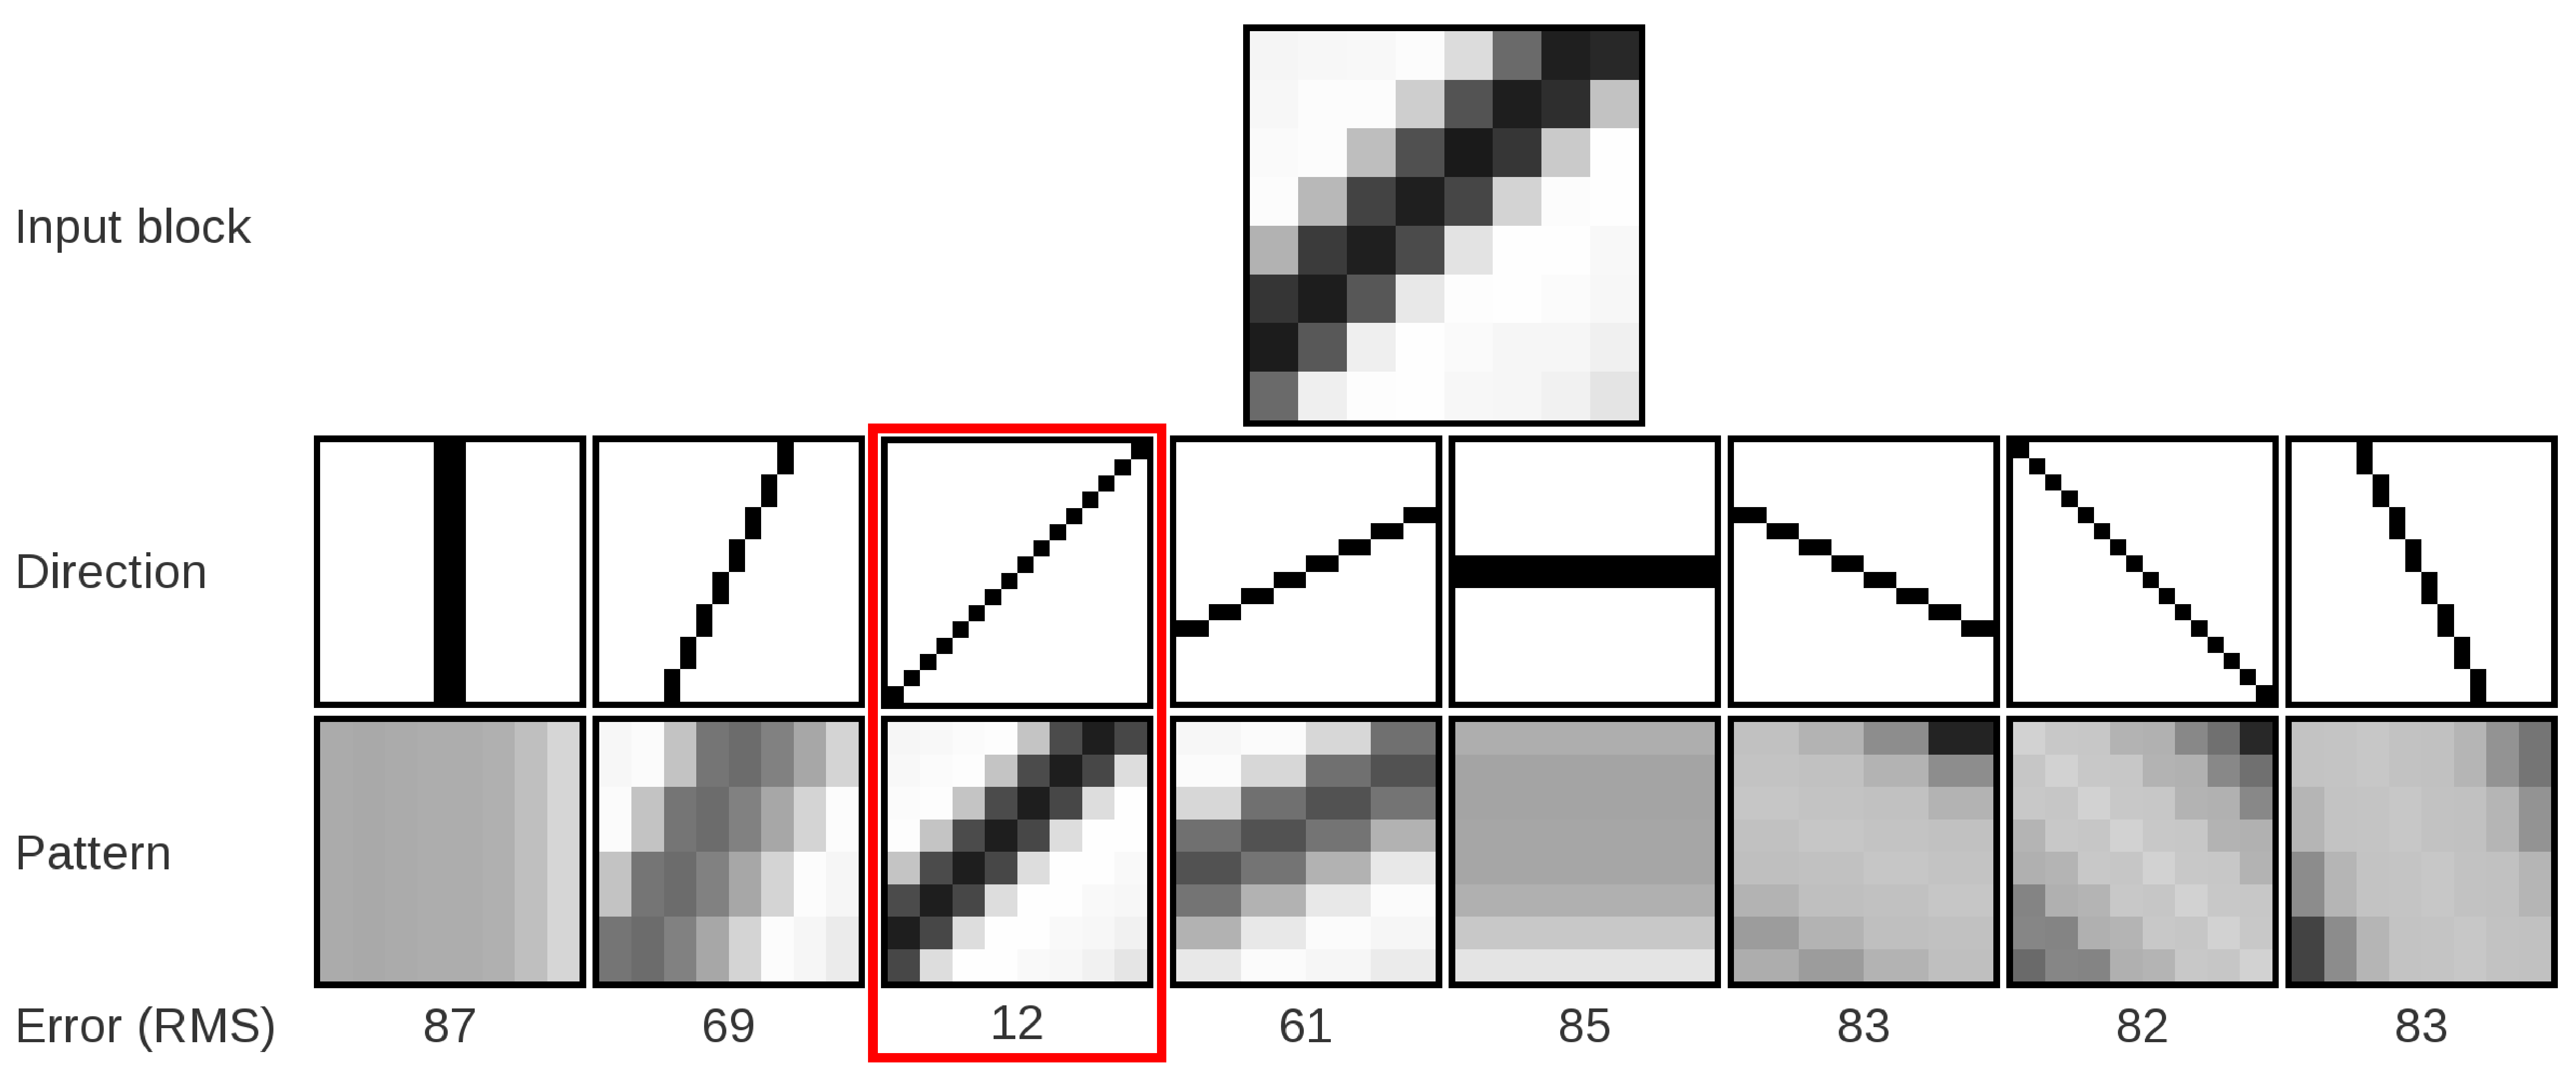
\includegraphics[width=1.0\columnwidth]{direction}}\caption{Example of direction search for an $8\times8$ block. The patterns
shown are based on the $\mu_{d,k}$ values. In this case, the 45-degree
direction is the one that minimizes $\sigma_{d}^{2}$, so it would
be selected by the search. Note that the error values $\sigma_{d}$
shown are never computed in practice (only $s_{d}$ is). \label{fig:Example-of-direction}}

\end{figure}

\begin{algorithm}[t]
\noindent\fbox{%
\begin{varwidth}{\dimexpr\linewidth-2\fboxsep-2\fboxrule\relax}
\begin{algorithmic}
\STATE {Initialize all variables to zero}
\FOR{$d=0$ to $7$}
  \FOR{$i=0$ to $7$}
    \FOR{$j=0$ to $7$}
      \STATE $L \leftarrow \mathrm{line\_table}[d][i][j]$
      \STATE $\mathrm{partial}[d][L] \leftarrow \mathrm{partial}[d][L] + \left(\mathrm{pixel}[i][j] - 128\right)$
      \STATE $\mathrm{count}[d][L] \leftarrow \mathrm{count}[d][L] + 1$
    \ENDFOR
  \ENDFOR
  \FOR{$L=0$ to $14$}
    \IF{$\mathrm{count}[d][L] > 0$}
      \STATE $s[d] \leftarrow s[d] + \mathrm{partial}[d][L]^2\cdot 840/\mathrm{count}[d][L]$
    \ENDIF
  \ENDFOR
\ENDFOR
\FOR{$d=0$ to $7$}
  \IF{$s[d] > s[\mathrm{best\_}d]$}
    \STATE $\mathrm{best\_}d \leftarrow d$ 
  \ENDIF
\ENDFOR
\STATE $\mathrm{direction} \leftarrow \mathrm{best\_}d$
\STATE $\mathrm{variance} \leftarrow s[\mathrm{best\_}d] - s[(\mathrm{best\_}d+4) \mod 8]$
\end{algorithmic}
\end{varwidth}% 
}
\caption{Direction search. The line\_table[$d$][$i$][$j$] values are the line numbers shown
in Fig.~\ref{fig:Lines-for-direction}. Note that in a practical implementation,
the $840/\mathrm{count}[d][L]$ term does not need to be computed, since it
only depends on $d$ and $L$\label{cap:direction-search}. Functionally equivalent algebraic simplifications
are possible, but they are not shown here for clarity.}
\end{algorithm}



\section{Non-linear Low-pass Filter}

\label{sec:nonlinear-lowpass}
CDEF is based on a non-linear low-pass filter designed to remove coding artifacts without
blurring sharp edges. This is achieved by selecting taps based on the
identified direction, but also by preventing excessive blurring when the filter
is applied across an edge. The latter is achieved through the use of a non-linear low-pass
filter that deemphasizes taps that differ too much from the pixel being filtered.
In one dimension, the non-linear filter can be expressed as
\begin{equation}
y\left(i\right)=x\left(i\right) +\!\!\sum_{m}w_k f\left(x\left(i+m) - x(i\right), S, D\right)\ ,\label{eq:linear-filter}
\end{equation}
where $w_k$ are the filter weights and $f(d, S, D)$ is a \textit{constraint function} operating
on the difference between the filtered pixel and each of the
neighbouring pixels. For small differences, $f\left(d, S, D\right)=d$, making the filter in
(\ref{eq:linear-filter}) behave like a linear filter. However, when the difference is large,
$f\left(d, S, D\right)=0$, which effectively ignores the filter tap.
The filter is parametrized by a \textit{strength} $S$ and a \textit{damping} value $D$:
\begin{equation}
f\left(d, S, D\right)=\left\{\begin{array}{ll}
\!\!\min\left(d, \max\left(0, S-\left\lfloor{\frac{d}{2^{D-\lfloor{\log_{2}S}\rfloor}}}\right\rfloor\right)\right) , d\ge0\\
\!\!\max\left(d, \min\left(0, \left\lceil{\frac{-d}{2^{D-\lfloor{\log_{2}S}\rfloor}}}\right\rceil-S\right)\right) , d<0
\end{array}\right. \label{eq:constraint-function}
\end{equation}
with $D \ge \lfloor\log_2{S}\rfloor$.
The strength $S$ controls the maximum difference allowed and the damping $D$ controls the point where
$f\left(d, S, D\right)=0$.  Fig.~\ref{fig:constraint-function-strength} illustrates
the effect of the strength on $f(\cdot)$ and Fig.~\ref{fig:constraint-function-damping}
illustrates the effect of damping. The function is anti-symmetric around $d=0$.



\begin{figure}
\centering{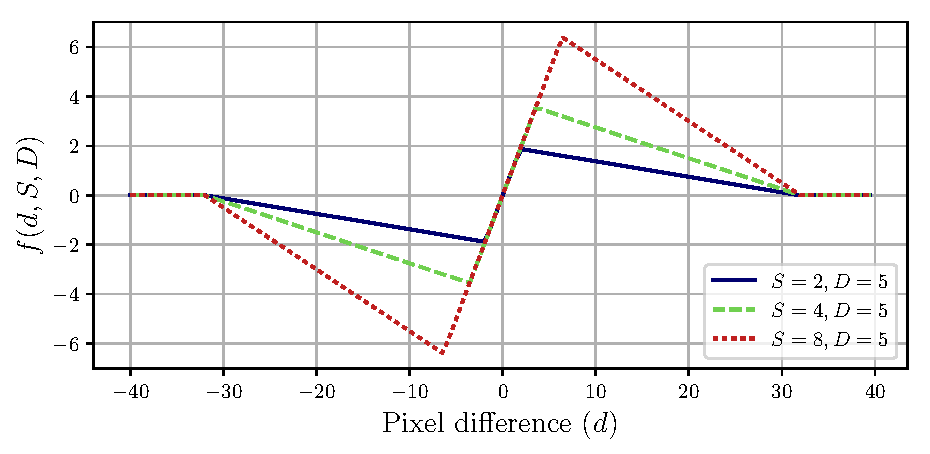
\includegraphics[width=0.9\columnwidth]{strength}}
\caption{Constraint function for different strength values $S$ (constant $D$).\label{fig:constraint-function-strength}}
\end{figure}


\begin{figure}
\centering{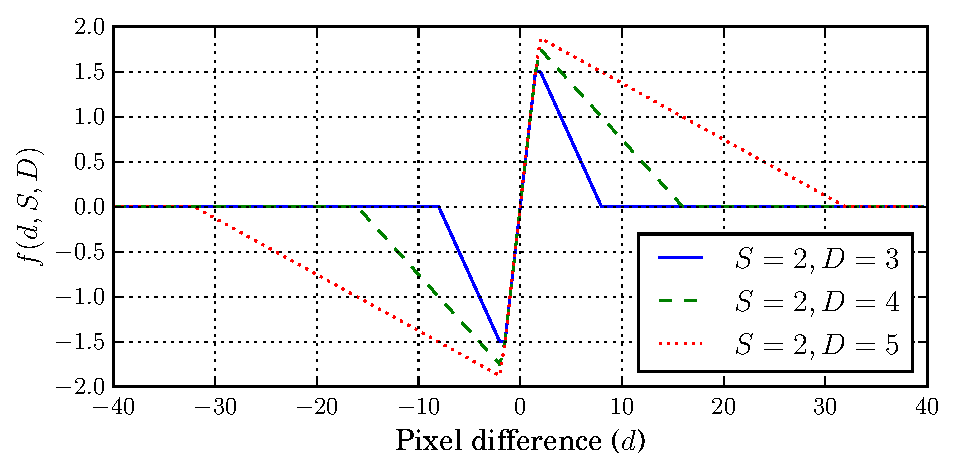
\includegraphics[width=0.9\columnwidth]{damping}}
\caption{Constraint function for different damping values $D$ (constant $S$).\label{fig:constraint-function-damping}}
\end{figure}

\subsection{Directional filter}

The main reason for identifying the direction of the Section~\ref{sec:direction-search} is to
align the filter taps along that direction to reduce ringing while preserving the directional
edges or patterns. However, directional filtering alone sometimes cannot
sufficiently reduce ringing so we also want to use filter taps on pixels that do not
lie along the main direction.
To reduce the risk of blurring, these extra taps are treated more conservatively. For this
reasons, CDEF defines \textit{primary taps} and \textit{secondary taps}. The primary taps follow
the direction $d$, and the weights are shown in Fig.~\ref{fig:Primary-filter}.  The weights for
the primary taps alternate for every other strength, so that the weights for strengths 1, 3, 5,
etc. are different from the weights for strengths 2, 4, 6, etc. This alternation is to be
preserved for higher bit depths (more than 8 bit).  The secondary taps
form a cross, oriented $45^\circ$ off the direction $d$ and their weights are shown in
Fig.~\ref{fig:Secondary-filter}. The complete 2-D CDEF filter is expressed as
\begin{align}
y\left(i, j\right)=&x(i, j) + \mathrm{round}\bigg( \nonumber\\
 & \sum_{m,n}{w}^{(p)}_{d,m,n}f\left(x\left(m, n) - x(i,j\right), S^{(p)}, D\right) \nonumber\\
+& \sum_{m,n}{w}^{(s)}_{d,m,n}f\left(x\left(m, n) - x(i,j\right), S^{(s)}, D\right) \bigg)\ ,
\label{eq:linear-filter2}
\end{align}
where $S^{(p)}$ and $S^{(s)}$ and the strengths of the primary and secondary taps, respectively,
and $\mathrm{round}(\cdot)$ rounds to the nearest integer, with ties away from zero.

Since the sum of all the primary and secondary weights exceed unity, it is possible (though rare) for
the output $y(i,j)$ to change by more than the maximum difference between the input and the neighbouring
values. This is avoided by explicitly clamping the filter output based on the neighbouring pixels with
non-zero weights:
\begin{align}
y_{clip}(i,j) &= \min\left(y_{max}, \max\left(y_{min}, y(i,j) \right) \right)\\
y_{min} &= \min_{m, n \in R}(x(i+m,j+n)) \\
y_{max} &= \max_{m, n \in R}(x(i+m,j+n)) \\
R &= (n,m) | {w}^{(p)}_{d,m,n}+{w}^{(s)}_{d,m,n} \ne 0
\label{eq:cap-function}
\end{align}

\begin{figure}
\centering{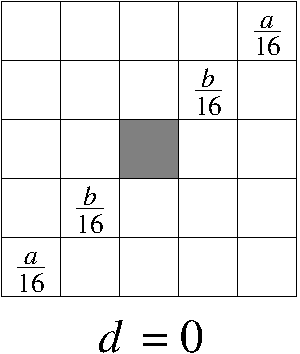
\includegraphics[width=0.24\columnwidth]{pri0}\hspace{.35em}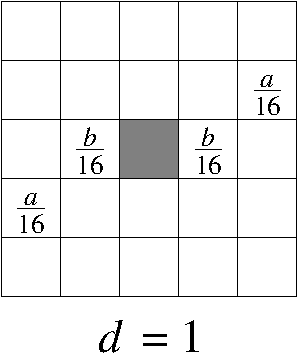
\includegraphics[width=0.24\columnwidth]{pri1}\hspace{.35em}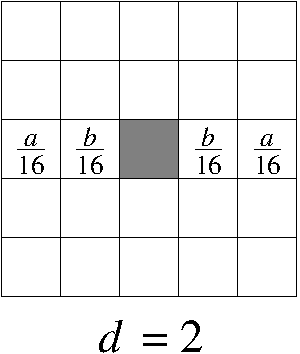
\includegraphics[width=0.24\columnwidth]{pri2}\hspace{.35em}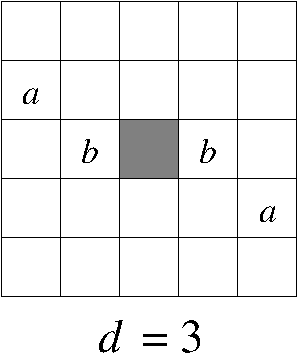
\includegraphics[width=0.24\columnwidth]{pri3}}

\vspace{.5em}

\centering{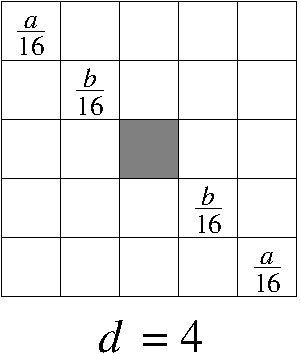
\includegraphics[width=0.24\columnwidth]{pri4}\hspace{.35em}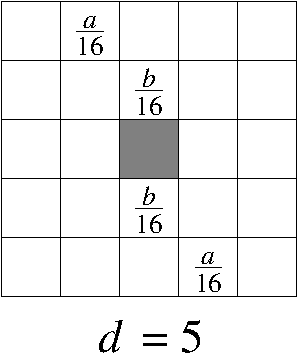
\includegraphics[width=0.24\columnwidth]{pri5}\hspace{.35em}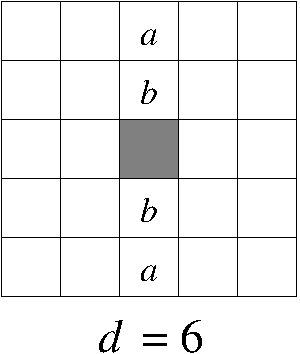
\includegraphics[width=0.24\columnwidth]{pri6}\hspace{.35em}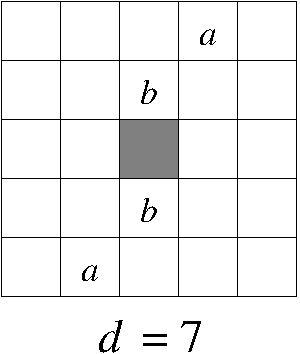
\includegraphics[width=0.24\columnwidth]{pri7}}
\caption{Primary filter taps following direction $d=0:7$. For even strengths $a=2$ and $b=4$, whereas for odd strengths $a=3$ and $b=3$.
The filtered pixel in shown in gray.
\label{fig:Primary-filter}}
\end{figure}


\begin{figure}
\centering{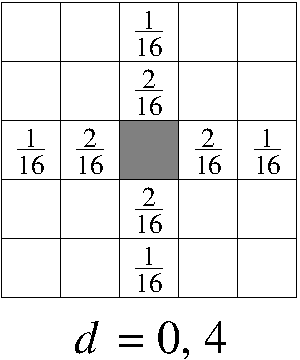
\includegraphics[width=0.24\columnwidth]{sec0}\hspace{.35em}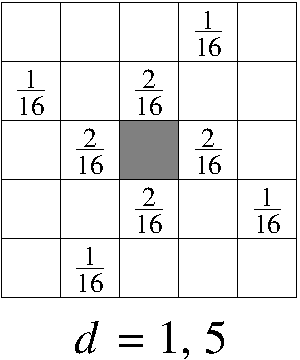
\includegraphics[width=0.24\columnwidth]{sec1}\hspace{.35em}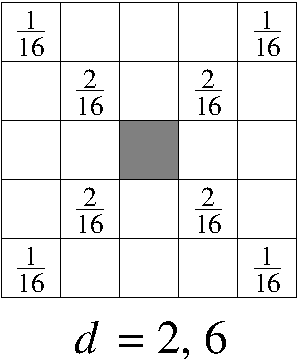
\includegraphics[width=0.24\columnwidth]{sec2}\hspace{.35em}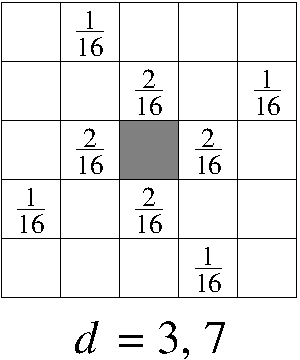
\includegraphics[width=0.24\columnwidth]{sec3}}
\caption{Secondary filter taps following direction $d=0:7$. The filtered pixel is shown in gray.\label{fig:Secondary-filter}}
\end{figure}

The direction, strength and damping parameters are constant over each $8\times8$
block being filtered. When processing the pixel at position $(i,j)$, the
filter is allowed to use pixels $x(i+m,j+m)$ lying outside of the
$8\times8$ block, or even outside of the superblock. If
the input pixel lies outside of the frame (visible area), then the pixel
is ignored, i.e. $f(d,S,D)=0$. To maximize parallelism, CDEF always operates
on the input (post-deblocking) pixels $x(i,j)$ so filtered pixels are never reused
for filtering other pixels.

\subsection{Valid strengths and damping values}

The strengths $S^{(p)}$ and $S^{(s)}$ and damping value $D$ must be set high
enough to smooth out coding artifacts, but low enough to avoid
blurring important details in the image.  For 8-bit content $S^{(p)}$ can
have integer values between $0$ and $15$, and $S^{(s)}$ can be $0$, $1$,
$2$ or $4$.  $D$ can be set to $3$, $4$, $5$ or $6$ for luma, and the
damping value for chroma is always one less.  The damping value shall
never be lower than the $\log_2 S$ to ensure that
the shift value used to compute $2^{D-\lfloor{\log_{2}S}\rfloor}$ in (\ref{eq:constraint-function}) never
becomes negative.  For instance, if for chroma $S^{(p)}=15$ and the luma damping is $3$,
the chroma damping shall also be $3$ (and not 2) because $\left\lfloor\log_2 S^{(p)}\right\rfloor=3$.

For higher bit depth (more than 8 bits), $S^{(p)}$ and $S^{(s)}$ are scaled according to
the extra bit depth, and $D$ is offset accordingly. For example, 12-bit
content can have $S^{(p)}$ values of $0$, $16$, $32$, $...$, $240$, and
the valid $D$ values are $7$, $8$, $9$ and $10$.  Picking an optimial
damping value is less critical for compression gains than picking the
optimal strengths.  $S^{(p)}$ and $S^{(s)}$ are chosen independently for
luma and chroma.

The signaled primary strength $S^{(p)}$ is adjusted for luma using a
variance $v$ (see algorithm~\ref{cap:direction-search}) for the $8\times8$ block as follows:
\begin{equation}
S^{(p)}_{adj}=\left\{ \begin{array}{ll}
\left\lfloor\frac{S^{(p)} \left(4 + \min\left(\left\lfloor \log_2\left\lfloor\frac{v}{2^{16}}\right\rfloor\right\rfloor, 12\right)\right) + 8}{16}\right\rfloor &, v \ge 2^{10}\\
0 &, \mathrm{otherwise}
\end{array}\right. \label{eq:strength-adjustment}
\end{equation}
This adjustment is not applied for chroma, nor for the secondary strength $S^{(s)}$.

\begin{table}
\caption{CDEF Bj{\o}ntegaard-delta~\cite{Testing-draft} rate for
the objective-1-fast test set in AWCY. The AV1 and Thor encoders were
tested for a high-latency (HL) configuration, a real-time, low-latency (LL)
configuration, as well as for low latency and low-complexity (LL+LC)\label{tab:bd-rate}.}
\centering{%
\setlength\tabcolsep{2.1pt}
\begin{tabular}{cccccc}
\hline 
\small{Encoding} & \small{PSNR} & \small{CIEDE} & \small{PSNR-HVS} & \small{SSIM} & \small{MS-SSIM}\tabularnewline
\hline 
AV1 HL & -1.08\% & -2.11\% & -0.15\% & -1.11\% & -0.44\%\tabularnewline
AV1 LL & -1.93\% & -2.88\% & -0.86\% & -1.96\% & -1.18\%\tabularnewline
AV1 LL + LC & -3.68\% & -4.54\% & -2.50\% & -4.15\% & -3.05\%\tabularnewline
\hline
Thor HL & -2.26\% & -3.13\% & -0.49\% & -2.75\% & -1.39\%\tabularnewline
Thor LL & -3.19\% & -5.18\% & -1.34\% & -3.31\% & -2.23\%\tabularnewline
Thor LL + LC & -6.17\% & -10.33\% & -4.13\% & -7.60\% & -6.11\%\tabularnewline
\hline 
\end{tabular}}
\end{table}


\begin{figure}
\centering{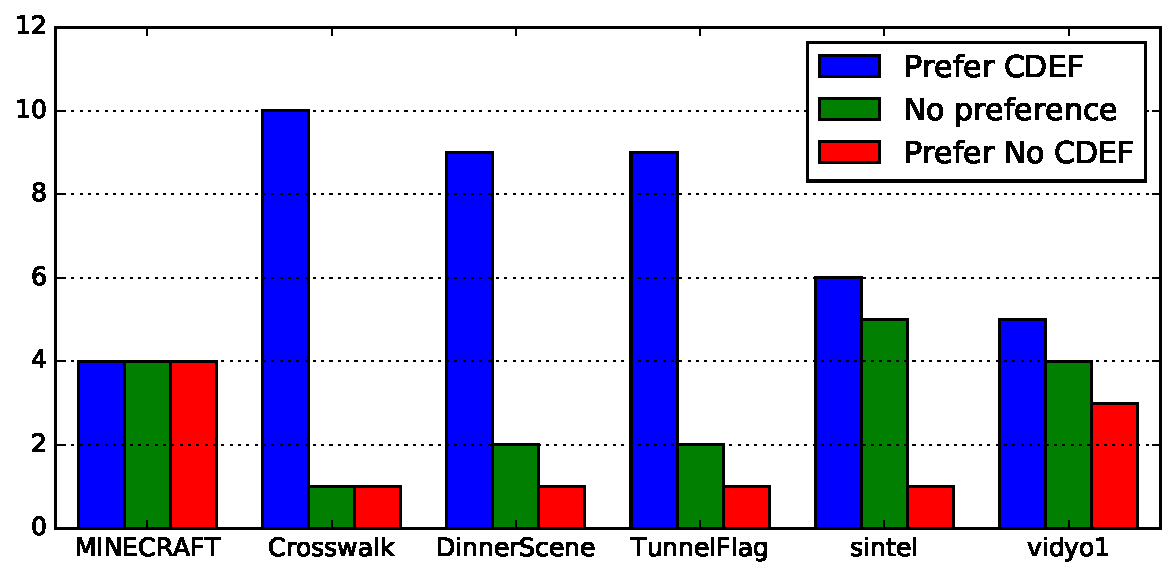
\includegraphics[width=\columnwidth]{cdef_vs_nothing}}
\caption{Subjective A-B comparison (with ties) results for CDEF vs. no processing for the high-latency configuration.\label{fig:subjective}}
\end{figure}


\section{Signaling and Filter Blocks}
\label{sec:signaling}

Some CDEF parameters are signaled at the frame level, and some
parameters may be signaled at the filter block ($64\times64$) level.  The following is
signaled at the frame level: the damping $D$ (2 bit), the number of
bits used for filter block signaling (0-3, 2 bits), and a list of 1, 2,
4 or 8 presets.  One preset contains the luma primary strength (4
bits), the chroma primary strength (4 bits), the luma secondary
strength (2 bits), the chroma secondary strength, a luma skip
condition bit, and a chroma skip condition bit (a total of 14 bits per
preset).  The filtering is applied one filter block at a time.  For each
filter block, the 0 - 3 bits are read to indicate the preset that will
be used for this filter block.  The filter
parameters are only coded for filter blocks that are not completely
skipped.  Such skipped filter blocks have CDEF disabled.
Similarly, any skipped coding block within a filter block has filtering
disabled unless the skip condition bit is set for that filter block.

Since the skip condition flag would be redundant in the case when both
the primary and secondary filter strengths are $0$, this combination
has a special meaning.  In that case, the
block shall be filtered with a primary filter strength equal to $19$
and a secondary filter strength equal to $7$.  The skip condition
flag is still to be regarded as $1$.

When the chroma subsampling differs horizontally and vertically,
e.g. 4:2:2 video, the filter is disabled for chroma, and the chroma
primary strength, the chroma skip condition flag and the chroma
secondary strength are not signaled.

\section{Encoder Search}
\label{sec:encoder-search}

On the encoder side, the search needs to determine both the frame level parameters
(preset parameters, number of presets) and the filter block-level preset ID. Assuming
the presets are already chosen, the ID for each non-skipped filter block is
chosen by minimizing a distortion metric over the filter block. The simplest error metric
is the sum of squared error (SSE), defined as $D=\left\Vert\mathbf{s}-\mathbf{d}\right\Vert^2$,
where $\mathbf{s}$ is a vector containing the source (uncoded) pixels for the filter block and
$\mathbf{d}$ contains the decoded pixels, filtered using a particular preset. While SSE leads
to good results overall, it sometimes causes excessive smoothing in non-directional textured
areas (e.g. grass). Instead, we use a modified version of SSE that takes into account
contrast in a similar way to the structural similarity (SSIM) metric~\cite{wang2004image}. The
distortion metric is the sum over the filter block of the following $8\times8$ distortion function:
\begin{equation}
D_{8\times8} = \frac{\sigma_s^2 + \sigma_d^2 + C_1}{2\sqrt{\sigma_s^2\sigma_d^2 + C_2}}\cdot\left\Vert\mathbf{s}-\mathbf{d}\right\Vert^2\ ,
\end{equation}
where $\sigma_s^2$ and $\sigma_d^2$ are the variances of $\mathbf{s}$ and $\mathbf{d}$ over the
block and the constants are set to $C_1=6.25$ and $C_2=312.5$ for 8-bit depth. Since the distortion
metric is only used in the encoder, it is not normative.

There are many possible strategies for choosing the presets for the frame, depending
on the acceptable complexity requirements and whether the encoder is allowed to make
two passes through the frame. In the two-pass case, the first step is to measure the
distortion $D_{b,p}$ for each filter block b, for each combination $p$ of 
$S^{(p)}$, $S^{(s)}$ and skip condition bit
($16\times4\times2=128$ parameter combinations) and for each plane. 
Once the distortion values are computed, the goal is to find the two sets of presets
$P_{\mathrm{luma}}$ and $P_{\mathrm{chroma}}$ that minimize the rate-distortion cost
\begin{equation}
J=\lambda B\log_2 N +  \sum_{b} \left(\min_{p \in P_{\mathrm{luma}}} D^{\mathrm{luma}}_{b,p} + \min_{p \in P_{\mathrm{chroma}}} D^{\mathrm{chroma}}_{b,p}\right)\ ,
\end{equation}
where $N$ is the cardinality of $P_{\mathrm{luma}}$ and $P_{\mathrm{chroma}}$ and $B$ is
the number of filter blocks. While we are not aware of polynomial-time algorithms to find the
global minimum, we have found that a greedy search can produce near-optimal results. With
the greedy search, we start by finding the optimal presets for $N=1$ and then increment $N$
by finding the optimal preset to add while keeping the already-selected presets $1..N-1$ constant.
If the encoder can afford the complexity, it is possible to improve on the purely
greedy search by iteratively re-optimizing one preset at a time.

The high complexity version of the search described above typically results in less than
1\% of the encoding time. Still, for low complexity operation, it is possible to reduce
the search complexity by only considering a subset of the 128 possible presets. 
This results in only a small loss ($<0.1\%$ BD-rate) in quality.

The damping value may be determined from
the quantizer alone (larger damping for larger quantizer).

\section{Results}
\label{sec:results}

We tested CDEF with the Are We Compressed
Yet~\cite{AWCY} online testing tool using the AV1 and Thor codecs, both
still in development at the time of writing. The results are shown in
Table~\ref{tab:bd-rate} for the objective-1-fast test set.  These
results reflect the gains in the codebases for git SHA's \texttt{e200b28}
(8th August 2017) and \texttt{b5e5cc5} (21st October 2017) for AV1 and Thor
respectively.

CDEF competes for the same gains as some other coding tools, in
AV1 in particular the dual\_filter tool and to a lesser degree motion\_var
and ext\_tx.  Disabling these tools in AV1 roughly doubles the CDEF gains.
The Thor codec lacks these tools.  In medium to low complexity encoder configurations
some tools while keeping CDEF enabled may give a good compexity/compression trade-off.

Subjective tests have shown a significant improvement in quality for
most types of video content, as shown in Fig.~\ref{fig:subjective}.


\section{Conclusion}

We have demonstrated an effective algorithm for removing coding
artifacts from coded images and videos. By taking into account the
direction of the patterns, the risk of blurring is reduced. Objective
results show a bit-rate reductions up to 4.5\% on AV1 and 11.3\% on Thor.

\section{Acknowledgments}

We would like to thank Thomas Daede for organizing the subjective test.

\bibliographystyle{IEEEtran}
\bibliography{daala}

\end{document}
